% Prezentacja - etap 2 (21.X), wersja skrócona (maks. 10 minut).
% Pełna wersja: prezentacja.tex.
% Kompilacja (XeLaTeX):  tectonic prezentacja_krotka.tex   albo   latexmk -xelatex prezentacja_krotka.tex
\documentclass[aspectratio=169,11pt]{beamer}

\usetheme[progressbar=frametitle,numbering=fraction]{metropolis}
\usepackage[polish]{babel}
\usepackage{booktabs}
\usepackage{tabularx}
\usepackage{listings}
\usepackage{xcolor}
\usepackage{tikz}
\usetikzlibrary{arrows.meta,positioning}

\graphicspath{{../diagramy/}{../mockup/}}
\newcolumntype{L}{>{\raggedright\arraybackslash}X}

\definecolor{ok}{HTML}{11804B}
\definecolor{bad}{HTML}{C0392B}
\definecolor{warn}{HTML}{A15C00}
\definecolor{acc}{HTML}{1F5EFF}
\newcommand{\good}[1]{\textcolor{ok}{#1}}
\newcommand{\bad}[1]{\textcolor{bad}{#1}}

\lstset{
  basicstyle=\ttfamily\footnotesize,
  keywordstyle=\color{acc}\bfseries,
  commentstyle=\color{gray},
  language=SQL,
  morekeywords={RETURNING,NOWAIT},
  columns=fullflexible,
  keepspaces=true,
  frame=none,
  backgroundcolor=\color{black!4},
  xleftmargin=4pt, framexleftmargin=4pt,
  extendedchars=true,
}

\title{System zapisów na zajęcia}
\subtitle{Etap 2: architektura, prototypy i struktury danych}
\author{Kamil Kręcigłowa \and Bartosz Królik \and Krzysztof Krówka}
\institute{Inżynieria Oprogramowania, zima 2026/2027}
\date{21 października 2026}

\begin{document}

\maketitle

\begin{frame}{Pokrycie wymagań}
  \footnotesize
  \begin{tabularx}{\textwidth}{@{}>{\raggedright}p{3.4cm}>{\raggedright}p{2.4cm}L>{\raggedright\arraybackslash}p{1.8cm}@{}}
    \toprule
    \textbf{Wymaganie} & \textbf{Przypadki} & \textbf{Tabele (ER)} & \textbf{Prototyp} \\
    \midrule
    ograniczona liczba miejsc & UC2, UC13 & \texttt{section.capacity}, \texttt{enrolled\_count}, \texttt{waitlist\_limit} & scen. 1, 5 \\
    katalog i harmonogram & UC1, UC11, UC12 & \texttt{course}, \texttt{section}, \texttt{lecturer}, \texttt{meeting}, \texttt{room}, \texttt{term}, \texttt{enrollment\_round} & scen. 6 \\
    różne rozmiary grup & UC12, UC13 & \texttt{section.capacity}, \texttt{section.kind}, \texttt{room.seats} & scen. 1, 4, 5 \\
    wymagania wstępne & UC3, UC11, UC15 & \texttt{course\_prerequisite}, \texttt{completed\_course} & scen. 2, 6 \\
    kolizje w harmonogramie & UC4, UC12 & \texttt{meeting} (dzień, godziny, parzystość) & scen. 3 \\
    listy oczekujących & UC5, UC7, UC9, UC18 & \texttt{waitlist\_entry}, \texttt{notification} & scen. 4, 5, 6 \\
    \bottomrule
  \end{tabularx}
\end{frame}

\begin{frame}[plain]
  \begin{tikzpicture}[remember picture, overlay]
    \node at (current page.center) {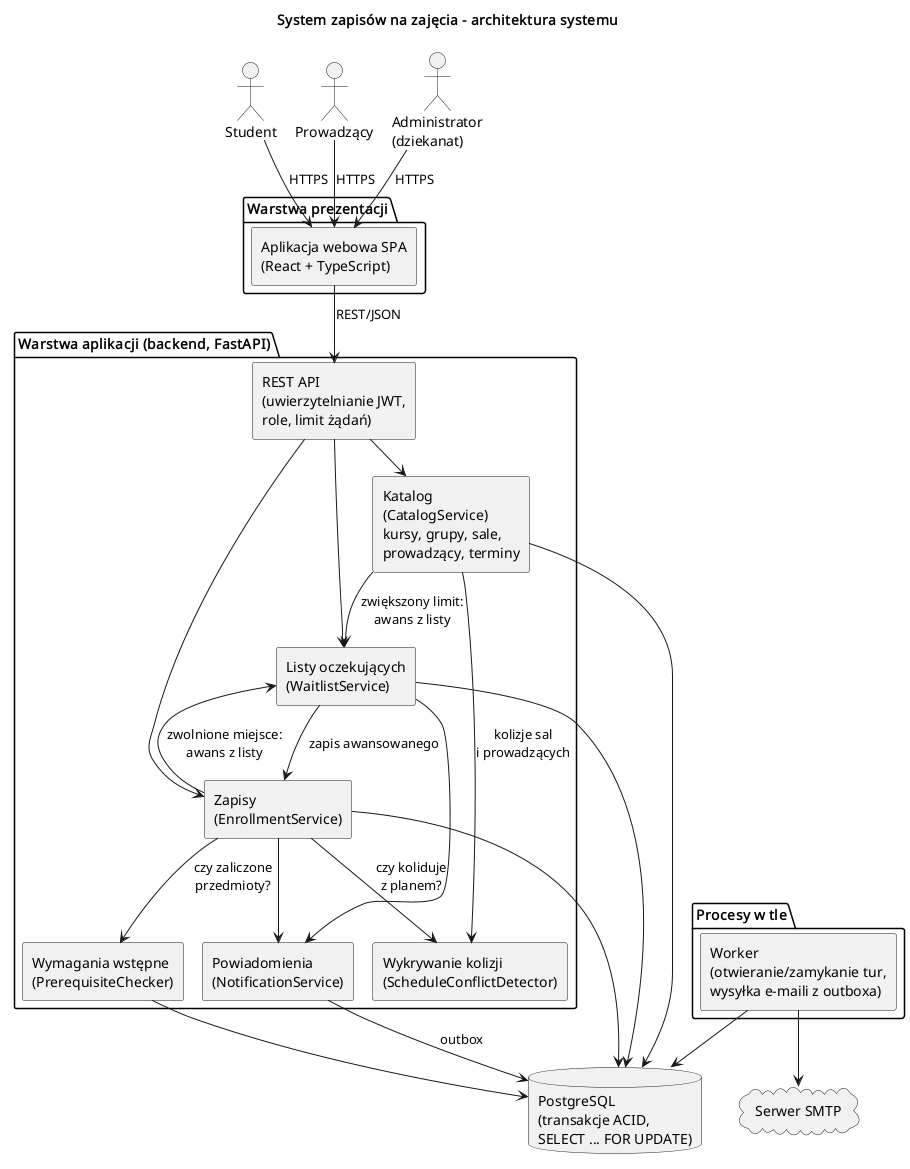
\includegraphics[height=0.98\paperheight]{architektura.png}};
  \end{tikzpicture}
\end{frame}

\begin{frame}{Architektura i stos technologiczny}
  \begin{columns}[T]
    \begin{column}{0.5\textwidth}
      \small
      \begin{itemize}
        \item \textbf{SPA} (React + TypeScript) dla studenta, prowadzącego, dziekanatu
        \item \textbf{REST API} (Python, FastAPI): JWT, role, limit żądań
        \item \texttt{EnrollmentService} -- \emph{jedyny} moduł zmieniający liczbę zajętych miejsc
        \item reguły: wymagania wstępne, kolizje; \texttt{WaitlistService}; outbox powiadomień
        \item \textbf{Worker}: tury zapisów, wygaszanie list, e-maile
        \item \textbf{PostgreSQL 16}: ACID, blokady wierszy, indeksy częściowe
      \end{itemize}
    \end{column}
    \begin{column}{0.46\textwidth}
      \begin{alertblock}{Główne wyzwanie}
        \small Otwarcie tury: setki studentów naraz walczą o te same miejsca.
      \end{alertblock}
      \small
      \begin{itemize}
        \item zapis do grupy serializuje blokada \textbf{wiersza grupy}
        \item zapisy jednego studenta -- blokada \textbf{wiersza studenta}
        \item różni studenci w różnych grupach -- równolegle
        \item outbox i tury w bazie $\Rightarrow$ bez osobnego brokera kolejek
      \end{itemize}
    \end{column}
  \end{columns}
\end{frame}

\begin{frame}{Przypadki użycia (1/2): student}
  \centering
  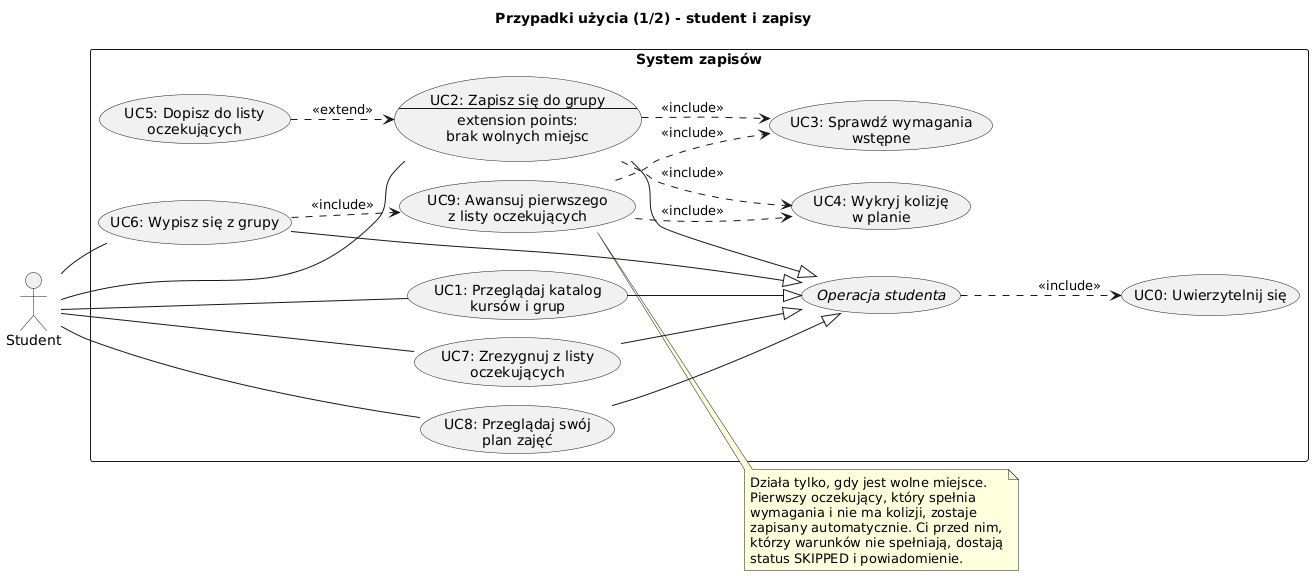
\includegraphics[height=0.86\textheight,width=\textwidth,keepaspectratio]{przypadki_uzycia_student.png}
\end{frame}

\begin{frame}{Przypadki użycia (2/2): dziekanat, prowadzący, zegar}
  \centering
  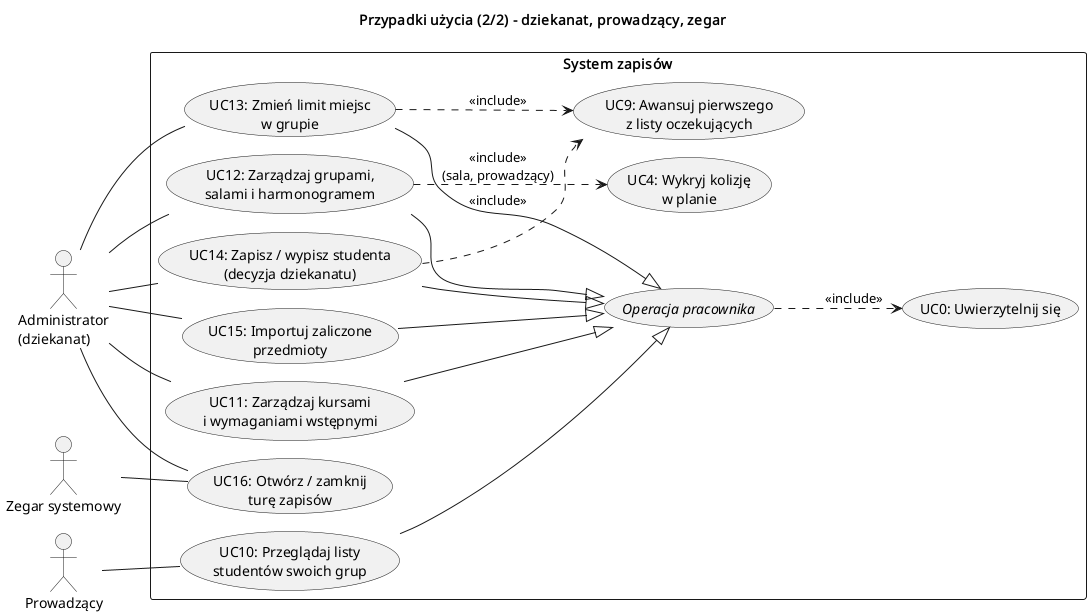
\includegraphics[height=0.86\textheight,width=\textwidth,keepaspectratio]{przypadki_uzycia_administracja.png}
\end{frame}

\begin{frame}{Kluczowe scenariusze: zapis i awans z listy}
  \begin{columns}[T]
    \begin{column}{0.5\textwidth}
      \small
      \textbf{UC2: Zapisz się do grupy}
      \begin{enumerate}
        \item Blokada studenta, potem grupy.
        \item Wymagania wstępne (UC3), kolizje (UC4), jedna grupa danego typu na przedmiot.
        \item Wolne miejsce $\Rightarrow$ zapis, licznik $+1$.
        \item Brak miejsc $\Rightarrow$ \textbf{UC5} (\texttt{<<extend>>}): koniec listy oczekujących.
      \end{enumerate}
      Każda odmowa podaje przyczynę (który przedmiot, z jaką grupą).
    \end{column}
    \begin{column}{0.46\textwidth}
      \small
      \textbf{UC9: Awans z listy}
      \begin{itemize}
        \item w \textbf{tej samej transakcji}, która zwolniła miejsce
        \item kolejni oczekujący sprawdzani \textbf{ponownie}; niespełniający $\Rightarrow$ \texttt{SKIPPED} + powiadomienie
        \item bez wolnego miejsca nikogo nie pomijamy
        \item zamknięcie tury $\Rightarrow$ listy wygasają
      \end{itemize}
      \begin{exampleblock}{Niezmiennik}
        Nikt nie czeka, gdy w grupie są wolne miejsca.
      \end{exampleblock}
    \end{column}
  \end{columns}
\end{frame}

\begin{frame}[plain]
  \begin{tikzpicture}[remember picture, overlay]
    \node at (current page.center) {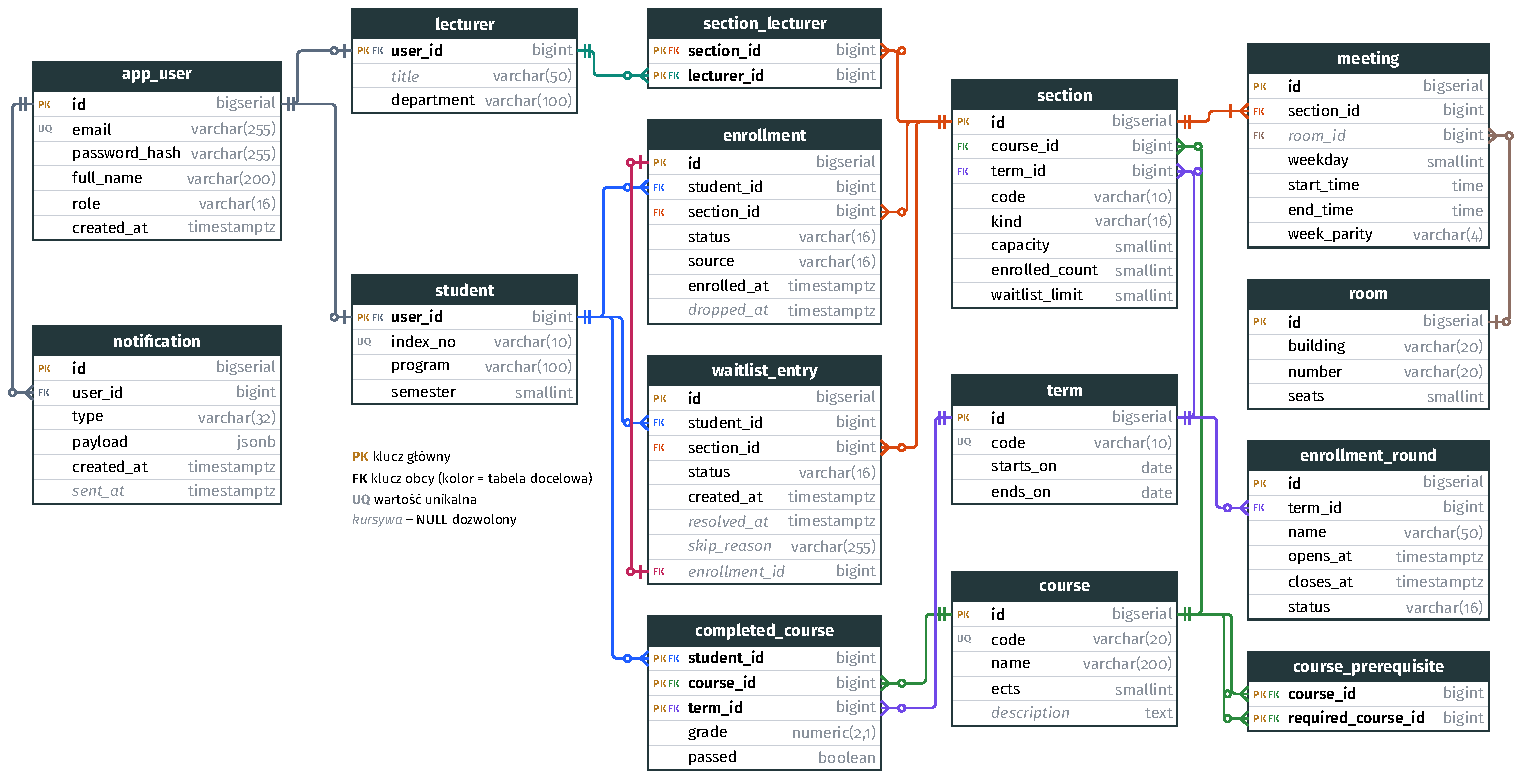
\includegraphics[width=0.99\paperwidth,height=0.98\paperheight,keepaspectratio]{er.pdf}};
  \end{tikzpicture}
\end{frame}

\begin{frame}[fragile]{Scenariusz 1: 30 studentów, 10 miejsc}
  \begin{columns}[T]
    \begin{column}{0.48\textwidth}
      \small
      \textbf{\bad{Wersja naiwna}}: odczyt licznika, potem osobny zapis
\begin{lstlisting}
SELECT enrolled_count, capacity ...
-- okno wyscigu
INSERT INTO enrollment ...
UPDATE section SET enrolled_count = :n+1
\end{lstlisting}
      \bad{30 zapisanych / 10 miejsc, licznik = 1}\\[3pt]
      \footnotesize \texttt{CHECK (enrolled\_count <= capacity)} tego \emph{nie} wykrywa -- licznik jest zaniżony.
      Wykrywa to widok \texttt{section\_invariant\_violations}.
    \end{column}
    \begin{column}{0.48\textwidth}
      \small
      \textbf{\good{Wersja bezpieczna}}: jedna atomowa operacja
\begin{lstlisting}
UPDATE section
   SET enrolled_count = enrolled_count + 1
 WHERE id = :section
   AND enrolled_count < capacity;
-- 0 wierszy => lista oczekujacych
\end{lstlisting}
      \good{10 zapisanych, 20 na liście, niezmienniki OK}\\[3pt]
      \footnotesize Wynik powtarzalny przy każdym uruchomieniu.
    \end{column}
  \end{columns}
\end{frame}

\begin{frame}[fragile]{Blokady w PostgreSQL: zakleszczenie przy awansie}
  \begin{columns}[T]
    \begin{column}{0.55\textwidth}
      \centering
      \begin{tikzpicture}[
          node distance=6mm,
          tx/.style={draw, rounded corners, minimum width=26mm, minimum height=7mm, font=\footnotesize, align=center},
          res/.style={draw, fill=black!6, minimum width=20mm, minimum height=7mm, font=\footnotesize},
          >={Stealth}]
        \node[tx] (t1) {Wypis A\\+ awans B};
        \node[tx, right=26mm of t1] (t2) {Zapis B\\do tej grupy};
        \node[res, below=12mm of t1] (sec) {grupa};
        \node[res, below=12mm of t2] (stB) {student B};
        \draw[->, ok, thick] (sec) -- node[left, font=\scriptsize]{trzyma} (t1);
        \draw[->, ok, thick] (stB) -- node[right, font=\scriptsize]{trzyma} (t2);
        \draw[->, bad, thick, dashed] (t1.south east) -- (stB.north west) node[pos=0.8, above right, font=\scriptsize]{czeka};
        \draw[->, bad, thick, dashed] (t2.south west) -- (sec.north east) node[pos=0.8, above left, font=\scriptsize]{czeka};
      \end{tikzpicture}\\[4pt]
      \footnotesize Sprawdzone na PostgreSQL 16 (dwie sesje):\\ \bad{\texttt{ERROR: deadlock detected}}
    \end{column}
    \begin{column}{0.41\textwidth}
      \small
      Zapis: \textbf{student $\to$ grupa}.\\
      Awans: \textbf{grupa $\to$ student B} -- odwrotnie.\\[4pt]
      \textbf{Rozwiązanie:}
\begin{lstlisting}
SELECT 1 FROM student
 WHERE user_id = :b
   FOR UPDATE NOWAIT;
\end{lstlisting}
      \footnotesize
      Zajęty $\Rightarrow$ błąd 55P03 od razu, \texttt{ROLLBACK} i ponowienie całej transakcji.
      B nie jest pomijany (nie traci kolejki). Tak samo obsługujemy 40P01 i 40001.
    \end{column}
  \end{columns}
\end{frame}

\begin{frame}{Mock-up: ekran zapisów studenta}
  \begin{columns}[T]
    \begin{column}{0.6\textwidth}
      \centering
      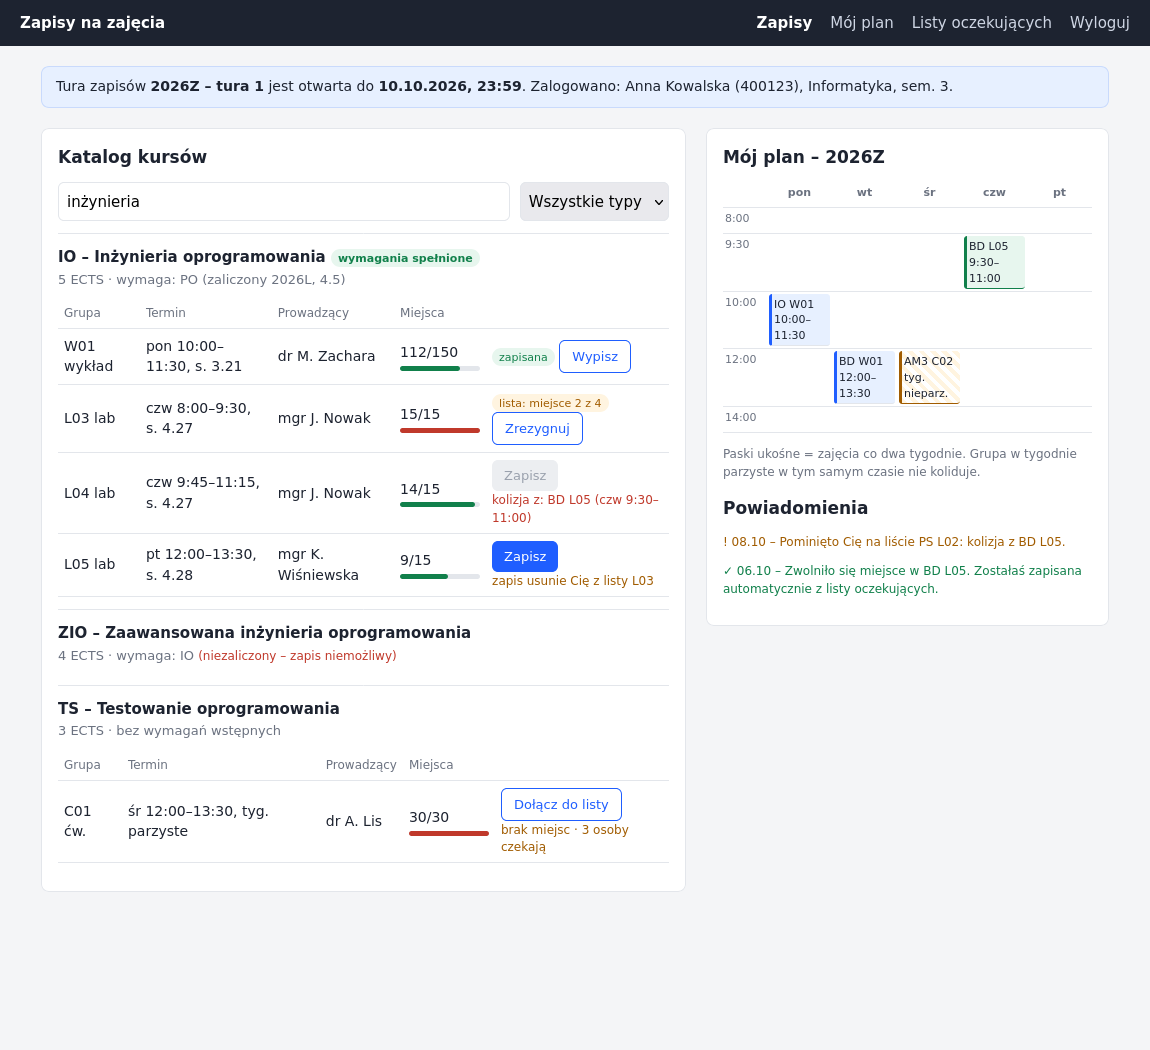
\includegraphics[height=0.84\textheight]{mockup.png}
    \end{column}
    \begin{column}{0.38\textwidth}
      \footnotesize
      \begin{itemize}
        \item katalog z zajętością miejsc
        \item kurs zablokowany przez niezaliczony przedmiot
        \item ,,Zapisz'' zablokowane przez kolizję, z podaniem grupy
        \item pozycja na liście, ,,Zrezygnuj'', ,,Dołącz do listy''
        \item ostrzeżenie: zapis usunie z listy innej grupy
        \item plan tygodnia z zajęciami co dwa tygodnie
        \item powiadomienia o awansie i pominięciu
      \end{itemize}
    \end{column}
  \end{columns}
\end{frame}

\begin{frame}{Podsumowanie}
  \begin{columns}[T]
    \begin{column}{0.5\textwidth}
      \small
      \textbf{Gotowe}
      \begin{itemize}
        \item architektura i stos technologiczny
        \item przypadki użycia UC0--UC18
        \item diagram ER + \texttt{schemat.sql} (PostgreSQL 16)
        \item prototyp 6 scenariuszy ryzyka
        \item mock-up ekranu zapisów
      \end{itemize}
    \end{column}
    \begin{column}{0.46\textwidth}
      \small
      \textbf{Etap 3 (28.X)}
      \begin{itemize}
        \item diagramy sekwencji
        \item diagram klas z metodami
        \item uprawnienia ról, obsługa błędów
        \item test blokad i wydajności
      \end{itemize}
    \end{column}
  \end{columns}
\end{frame}

\begin{frame}[standout]
  Dziękujemy!\\[6pt]
  \normalsize Pytania?
\end{frame}

\end{document}
